\chapter{Problem domain analysis}\label{ch:problemanalysis}
This chapter contains a problem domain analysis of how Labelless Medias handles leads. The purpose of the chapter is to identify and model the problem domain to get an understanding of the real world problems which the system should be capable of handling. The problem domain analysis includes the following four steps:
\begin{itemize}
  \item Establishing classes and events
  \item Creating an Event table
  \item Creating a diagram of class relations in the problem domain
  \item Describing the behavior model of the classes
\end{itemize}
\noindent

\section{Classes}
The first step of the problem domain analysis is to establish which classes ought to be included in the model of the problem domain. These classes should have a real world counterpart. The classes that have been established in the problem domain are described in this section.

\subsection{Client}
The class \textit{client} represents Labelless Media's clients. 
An object of this class, contains information about the client and an overview of the leads that the client has sent to Labelless Media. 

\subsection{Salesperson}
The \textit{salesperson} class represents an employee at Labelless Media who decides which leads to contact.
The salesperson can also cold call potential clients. If the cold call is successful, the salesperson is then responsible for inputting the lead and the client into the system.
When the salesperson has successfully contacted a client, the salesperson is assigned as the contact person to the \textit{client}.

\subsection{Lead}
The class \textit{lead} portrays a potential opportunity that could result in a contract for Labelless Media. An object of the class contains the client's answers to the questions in the contact form that is found on Labelless Media's website, see section \ref{ch:case}. This information is used to evaluate the attractiveness of the \textit{lead}. The attractiveness helps Labelless Media to determine whether or not they want to follow the lead. A lead can also be created by a salesperson, after successfully calling a potential client. In this case the salesperson fills in the information about the client. A \textit{lead} can be in different stages throughout its lifetime. The first stage is only for the leads that arrive through the contact form on Labelless Medias website. In this stage the lead is waiting to be followed, and moves to the second state when a salesperson, follows it and sets up a meeting. In this state, the \textit{lead} is responsible for keeping track of when the next meeting with a clients is, and alerting the responsible salesperson when a meeting draws close. When a contract with the client is made, the leads get marked as done, and is then archived in the system.

\subsection{Meeting}
The class \textit{meeting} represents a meeting that has been setup by a salesperson with a client about a lead. A meeting requires the salesperson, and a client before it can exist. An object of this class contains information about the meeting i.e.\ date, time and product.


\subsection{Problem domain class diagram}
\noindent
To get a better overview of the relations between the different classes within the problem domain, a class diagram is made. This is shown in Figure \ref{fig:ClassOverview}. 
The \textit{Lead} class is the heart of the class diagram. The remaining classes: \textit{Client}, \textit{Meeting} and \textit{Salesperson} all revolve around \textit{Lead} and have relations with the \textit{Lead} class. 

\begin{figure}[H]
    \centering
    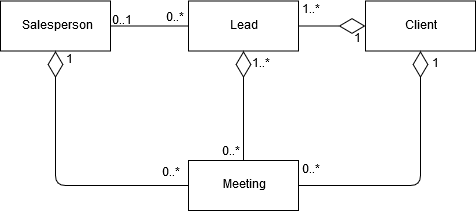
\includegraphics[scale=0.7, clip]{figures/ClassDiagrams/ProblemDomain.png}
    \caption{Class diagram of problem domain classes}
    \label{fig:ClassOverview}
\end{figure}
\noindent
A Lead is aggregated by a Client. For every Client there is at least one lead. A Client can have one to many Leads, but a Lead can only be connected to one Client. The Salesperson and the Lead is associated with each other, meaning that a Lead does not always belong to a Salesperson. When a Lead enters the system, it is not assigned to any Salesperson. A Lead is assigned to a Salesperson when the Salesperson reserves the lead. After a lead is has been assigned, only the Salesperson the Lead belongs to can change the lead. A meeting aggregates both one Client, one Lead and one Salesperson since the meeting is about a Lead and the attendees is the Salesperson assigned to the Lead, and the Client. Each of these three objects can have zero to many meetings. The reason why it is possible to have zero meetings, is because if a Lead gets declined, a meeting will not be necessary. 


\section{Events}
The classes for the problem domain has been established, and the next step in the problem domain analysis is to establish which events influence the objects of the classes. The events express the dynamics of the system.

\subsection{Event table}
After examining the classes and their events within the problem domain, an event table has been produced to better understand the relation between the classes and the events. In the event table in Figure \ref{tab:EventTable} a '+' sign indicates that the event can occur zero or one time. The '*' sign indicates that the event can occur zero or many times. The events that might not be self explanatory are described below.

\begin{table}[H]
\begin{tabular}{|l|l|l|l|l|l|l|}
\hline
\textbf{Event/Classes}    & Client & Meeting   & Lead  & Salesperson
\\ \hline
Lead created       &        &                 & +       &
\\ \hline
Lead reserved by salesperson     
                    &       &       & +       & *
\\ \hline
Lead accepted       &       &       & +       & * 
\\ \hline
Lead declined       &       &       & +       & *
\\ \hline
Lead completed      &       &       & +       & *
\\ \hline
Lead deleted        &       &       & +       & *
\\ \hline
Client created      & +      &      &         &   
\\ \hline
Client contacted    & *      &      &  +      & *
\\ \hline
Client deleted      & +      &      &  +      &       
\\ \hline
Client flagged      & *      &      &         & *      
\\ \hline
Client unflagged    & *      &      &         & *     
\\ \hline
Salesperson hired   &        &      &         & +      
\\ \hline
Salesperson fired   &        &      &         & +     
\\ \hline
Meeting created     &  *     &   +  &     *   & *
\\ \hline
Meeting completed   &  *     &   +   &     *   &*
\\ \hline
Meeting canceled    &  *     &    +  &    *    & *
\\ \hline
\end{tabular}
\caption{Event table for the classes within the problem domain}
\label{tab:EventTable}
\end{table}

Lead reserved by salesperson is the event that occurs when a salesperson chooses to work together with a potential client. Also, this event prevent other salespersons from taking the same job and can therefore affect the statistics of the individual salesperson.
There is a difference between the two events Lead declined and Lead deleted. Lead declined is when the salesperson does not accept the lead. Here the lead still influences the algorithm that ranks all the leads. On the contrary, the event Lead deleted is when the salesperson removes the lead from the system and thus it does not affect the ranking system.

\section{Behavior models}
To get a better understanding of the respective life cycles of the classes, the events of the classes are displayed as state chart diagrams. These diagrams illustrate the behavioral patterns of the classes. 
\newline \newline \noindent
\textbf{Client}
\\
Figure \ref{fig:behaviourClient} shows a state diagram of a client object. It shows that the client has two states, flagged and unflagged. If a client is flagged, it indicates that the client is a bad payer. In both states, the client class can be contacted and a meeting can be made and completed.
Deletion of a client will usually only happen if it is required by the law or if it is requested by the client itself.
 
\begin{figure}[H]
    \centering
    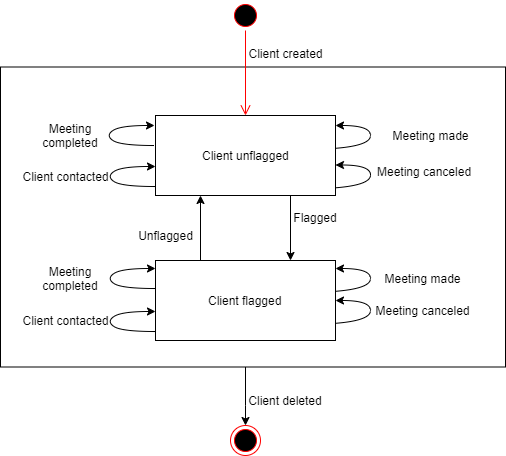
\includegraphics[scale=0.8, clip]{figures/Behaviors/BehaviorClient.png}
    \caption{The behaviour of a client }
    \label{fig:behaviourClient}
\end{figure}
\noindent
\noindent
\textbf{Lead}
\\
Figure \ref{fig:behaviourLead} illustrates the behavior of a \textit{lead}. It shows the four states a \textit{lead} can be in, where the first is before the lead has been reserved by a salesperson. In this state the \textit{lead} is ranked by the system and compared to all the other leads, until the leads gets reserved by a salesperson. The lead then moves to the second stage, until the client has been contacted. After contact with the client has been established, meetings can be made until either a contract is made or the lead gets denied. When the contract is made, the relevant earnings are entered into the system and lead is finished.

\begin{figure}[H]
    \centering
    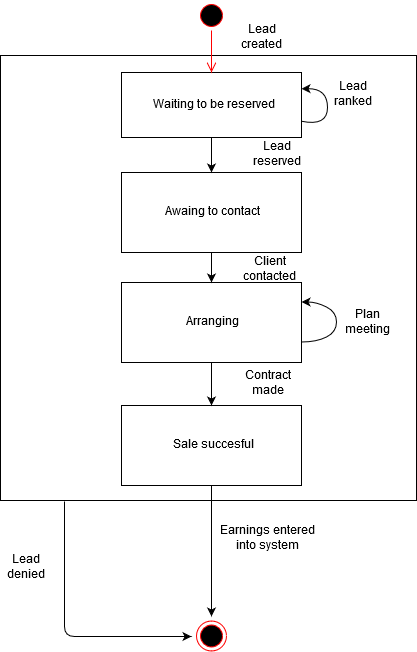
\includegraphics[scale=0.8, clip]{figures/Behaviors/BehaviorLead.png}
    \caption{The behaviour of a lead}
    \label{fig:behaviourLead}
\end{figure}


\noindent
\textbf{SalesPerson}
\\
Figure \ref{fig:behaviourSalesperson} illustrates the behavior of a salesperson. The salesperson can reserve, accept, decline, delete, and mark leads as completed. These events are all related to how a salesperson can interact with leads, for simplicity these actions are all grouped together under "Lead actions" in the behaviour model. When a salesperson reserves a lead, the lead is now bound to this salesperson. This salesperson is now marked as the owner of the lead, and his colleagues now knows that this lead is already being investigated by someone else. The behaviour model also shows a grouping of "Client actions" and "Meeting actions". The "Client actions" grouping consists of client contacted, client flagged, and client unflagged. The final grouping of "Meeting actions" consists of meeting created, meeting completed, and meeting cancelled. The salesperson ceases to exist when he is fired.


\begin{figure}[H]
    \centering
    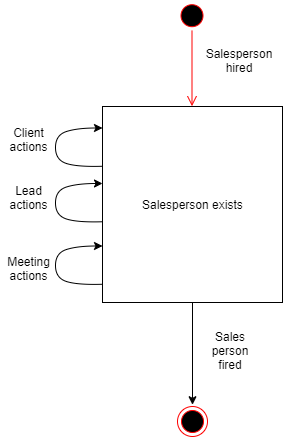
\includegraphics[scale=0.8, clip]{figures/Behaviors/BehaviorSalesPerson.png}
    \caption{The behaviour of a salesperson }
    \label{fig:behaviourSalesperson}
\end{figure}

\noindent
\textbf{Meeting}
\\
Figure \ref{fig:behaviourMeeting} illustrates the behaviour of a meeting. The \textit{Meeting} class simply represents a real life meeting between a salesperson from Labelless Media and a client. After a meeting is created it can only be completed or cancelled, which also leads to the ending of a meeting object. 
\begin{figure}[H]
    \centering
    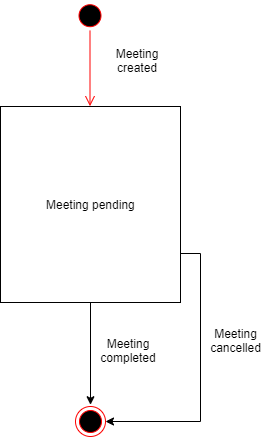
\includegraphics[scale=0.9, clip]{figures/Behaviors/BehaviorMeeting.png}
    \caption{The behaviour of a meeting }
    \label{fig:behaviourMeeting}
\end{figure}
\noindent



\section{Summary}
Der skal skrives en afrunding af kap. her


%\noindent
%Finally the behaviour of an evaluator can be seen in Figure \ref{fig:evaluatorBehaviour}. An evaluator is responsible for sorting archive data and ranking new leads based on the form. The new leads are ranked by an algorithm in the evaluator class. Leads are ranked to find the most promising ones. Leads are ranked based on user input. The existing archive of clients and leads can also be sorted by an algoritm within the evaluator object.

%\begin{figure}[H]
 %   \centering
  %  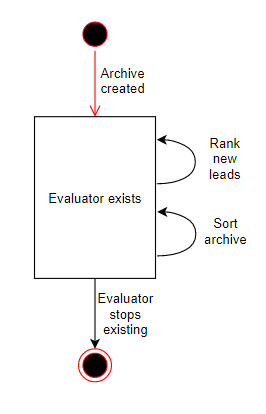
\includegraphics[scale=0.9, clip]{figures/evaluatorBehaviour.png}
  %  \caption{The behaviour of an evaluator }
   % \label{fig:evaluatorBehaviour}
%\end{figure}

